\subsection{Single Pod}
\subsubsection{Single Pod CPU Utilization}
\begin{itemize}
    \item CPU utilization in the Single Pod configuration can be relatively stable, as all workload is handled by a single pod.
    \item The pod may experience higher CPU usage during peak demand since it manages all requests.
    \item Over time, as workloads fluctuate, CPU usage may stabilize as the single pod adjusts to the demand.
\end{itemize}

\noindent Below is the graph that illustrates the CPU utilization for Single Pod:

\begin{figure}[h]
    \begin{minipage}[t]{0.5\textwidth}
        \centering
        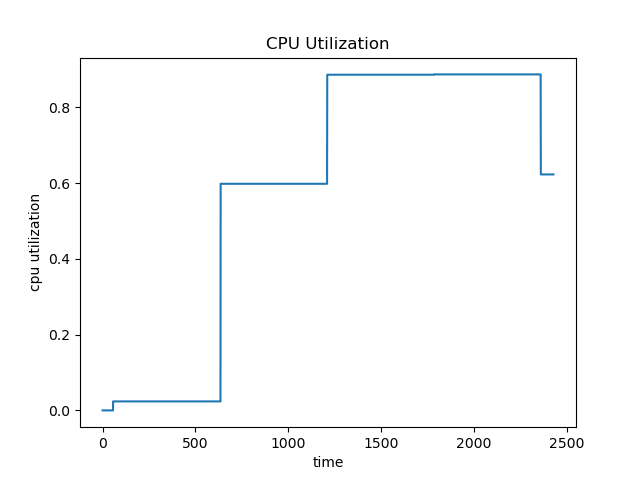
\includegraphics[width=0.9\textwidth]{../sample_results/loop/single-pod/cpu-utilization-single-pod.png}
        \caption{Loop}
    \end{minipage}
    \hfill
    \begin{minipage}[t]{0.5\textwidth}
        \centering
        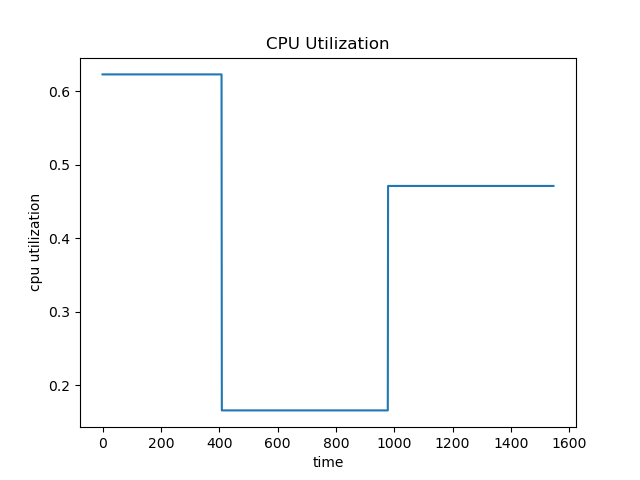
\includegraphics[width=0.9\textwidth]{../sample_results/lorem/single-pod/cpu-utilization-single-pod.png}
        \caption{Lorem}
    \end{minipage}
\end{figure}

\newpage
\subsubsection{Single Pod Response Time Observations}
\begin{itemize}
    \item Response times in the Single Pod configuration can be consistent, as a single pod handles all requests.
    \item Under heavy load, response times may increase due to the single pod being responsible for all tasks.
    \item As workloads stabilize, response times tend to remain steady, provided the pod is not overwhelmed.
\end{itemize}

\noindent Below are the response time graphs for Single Pod:

\begin{figure}[h]
    \begin{minipage}[t]{0.5\textwidth}
        \centering
        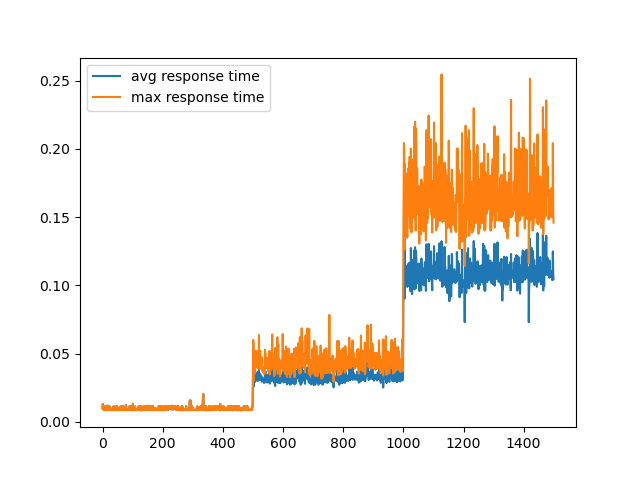
\includegraphics[width=0.9\textwidth]{../sample_results/loop/single-pod/response-time-single-pod-single-pod.png}
        \caption{Loop}
    \end{minipage}
    \hfill
    \begin{minipage}[t]{0.5\textwidth}
        \centering
        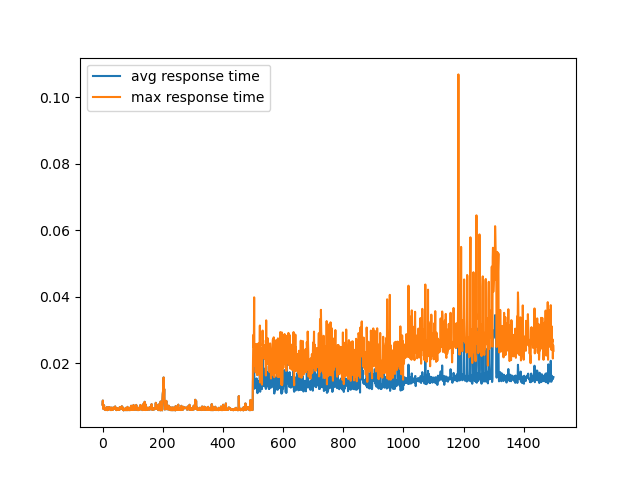
\includegraphics[width=0.9\textwidth]{../sample_results/lorem/single-pod/response-time-single-pod-single-pod.png}
        \caption{Lorem}
    \end{minipage}
\end{figure}

\newpage
\subsubsection{Single Pod Memory Utilization}
\begin{figure}[h]
    \begin{minipage}[t]{0.5\textwidth}
        \centering
        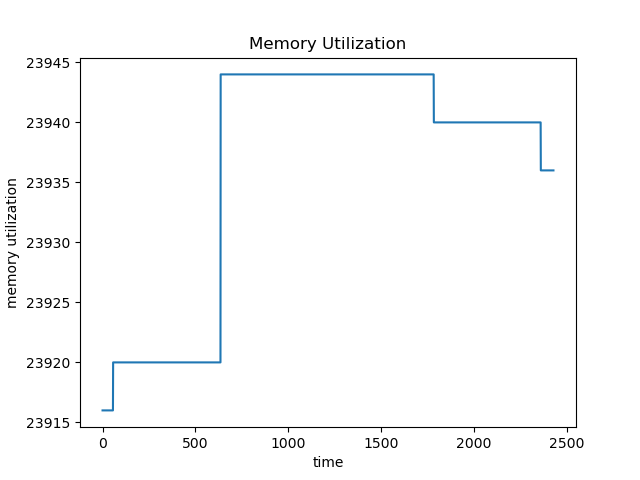
\includegraphics[width=0.9\textwidth]{../sample_results/loop/single-pod/mem-utilization-single-pod.png}
        \caption{Loop}
    \end{minipage}
    \hfill
    \begin{minipage}[t]{0.5\textwidth}
        \centering
        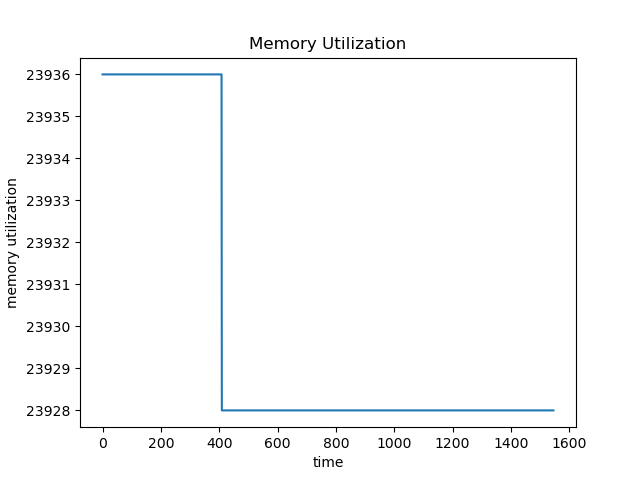
\includegraphics[width=0.9\textwidth]{../sample_results/lorem/single-pod/mem-utilization-single-pod.png}
        \caption{Lorem}
    \end{minipage}
\end{figure}

\begin{itemize}
    \item Memory utilization in the Single Pod configuration can vary based on the complexity of the workloads.
    \item The single pod manages memory allocation for all requests, which can lead to fluctuations in memory usage.
    \item As workloads stabilize, memory utilization tends to even out, provided the single pod is adequately resourced.
\end{itemize}

